\documentclass{beamer}
\usepackage[utf8]{inputenc}
\usepackage[spanish]{babel}
\usepackage{amsmath}
\usepackage{graphicx}
\usepackage{hyperref}
\usetheme{Madrid}

% Eliminar el pie de página
\setbeamertemplate{footline}{} % <-- esto elimina completamente el pie

% Cabecera personalizada (solo encabezado)
\setbeamertemplate{headline}{
  \leavevmode%
  \hbox{%
  \begin{beamercolorbox}[wd=0.5\paperwidth,ht=2.5ex,dp=1.5ex,center]{author in head/foot}%
    \textbf{Métodos de Optimización}
  \end{beamercolorbox}%
  \begin{beamercolorbox}[wd=0.5\paperwidth,ht=2.5ex,dp=1.5ex,center]{title in head/foot}%
    Universidad Nacional del Altiplano - FINESI
  \end{beamercolorbox}}%
}

% Datos de portada
\title{Aplicación de la Programación Lineal en la Generación de Horarios Escolares}
\subtitle{Basado en el artículo:\\ \textit{Development of a tool to schedule school timetabling through linear programming}}
\author{Beatriz Umiña Machaca \\ Código: 230035}
\date{6 de mayo de 2025}

\begin{document}

% 1. Portada
\begin{frame}
  \titlepage
\end{frame}
h
% 2. Introducción
\begin{frame}{¿Por qué se usó programación lineal?}
  \begin{itemize}
    \item Crear horarios manualmente era lento (13 horas por semana en el colegio HS).
    \item Se buscaba una solución automática, rápida y sin errores.
    \item La programación lineal permite modelar reglas y restricciones con precisión.
  \end{itemize}
\end{frame}

% 3. ¿Qué es la programación lineal?
\begin{frame}{¿Qué es la programación lineal?}
  \begin{itemize}
    \item Es una técnica matemática que optimiza una función respetando restricciones.
    \item Usa variables de decisión, restricciones y una función objetivo.
    \item En este caso se aplicó \textbf{programación lineal entera binaria}.
    \item Ideal para horarios: 1 clase = 1 hora, sí o no (binaria).
  \end{itemize}
\end{frame}

% 4. Modelo matemático
\begin{frame}{Modelo aplicado}
  \begin{itemize}
    \item Variables binaria: $x_{p,c,h,s} = 1$ si el profesor \( p \) da el curso \( c \) en hora \( h \) en salón \( s \).
    \item Restricciones:
      \begin{itemize}
        \item No solapamiento de clases ni profesores.
        \item Horas necesarias por materia.
        \item Disponibilidad de salones y docentes.
      \end{itemize}
    \item Se definieron más de 100 mil restricciones en total.
  \end{itemize}
\end{frame}

% 5. Herramienta y resultados
\begin{frame}{Solución y resultados}
  \begin{itemize}
    \item Se implementó el modelo en \textbf{Excel} usando \textbf{OpenSolver}.
    \item Se ingresaron todas las variables, restricciones y objetivos.
    \item Tiempo de cálculo: \textbf{1.37 horas}.
    \item Resultado: horarios funcionales y validados.
\begin{figure}[H]
    \centering
    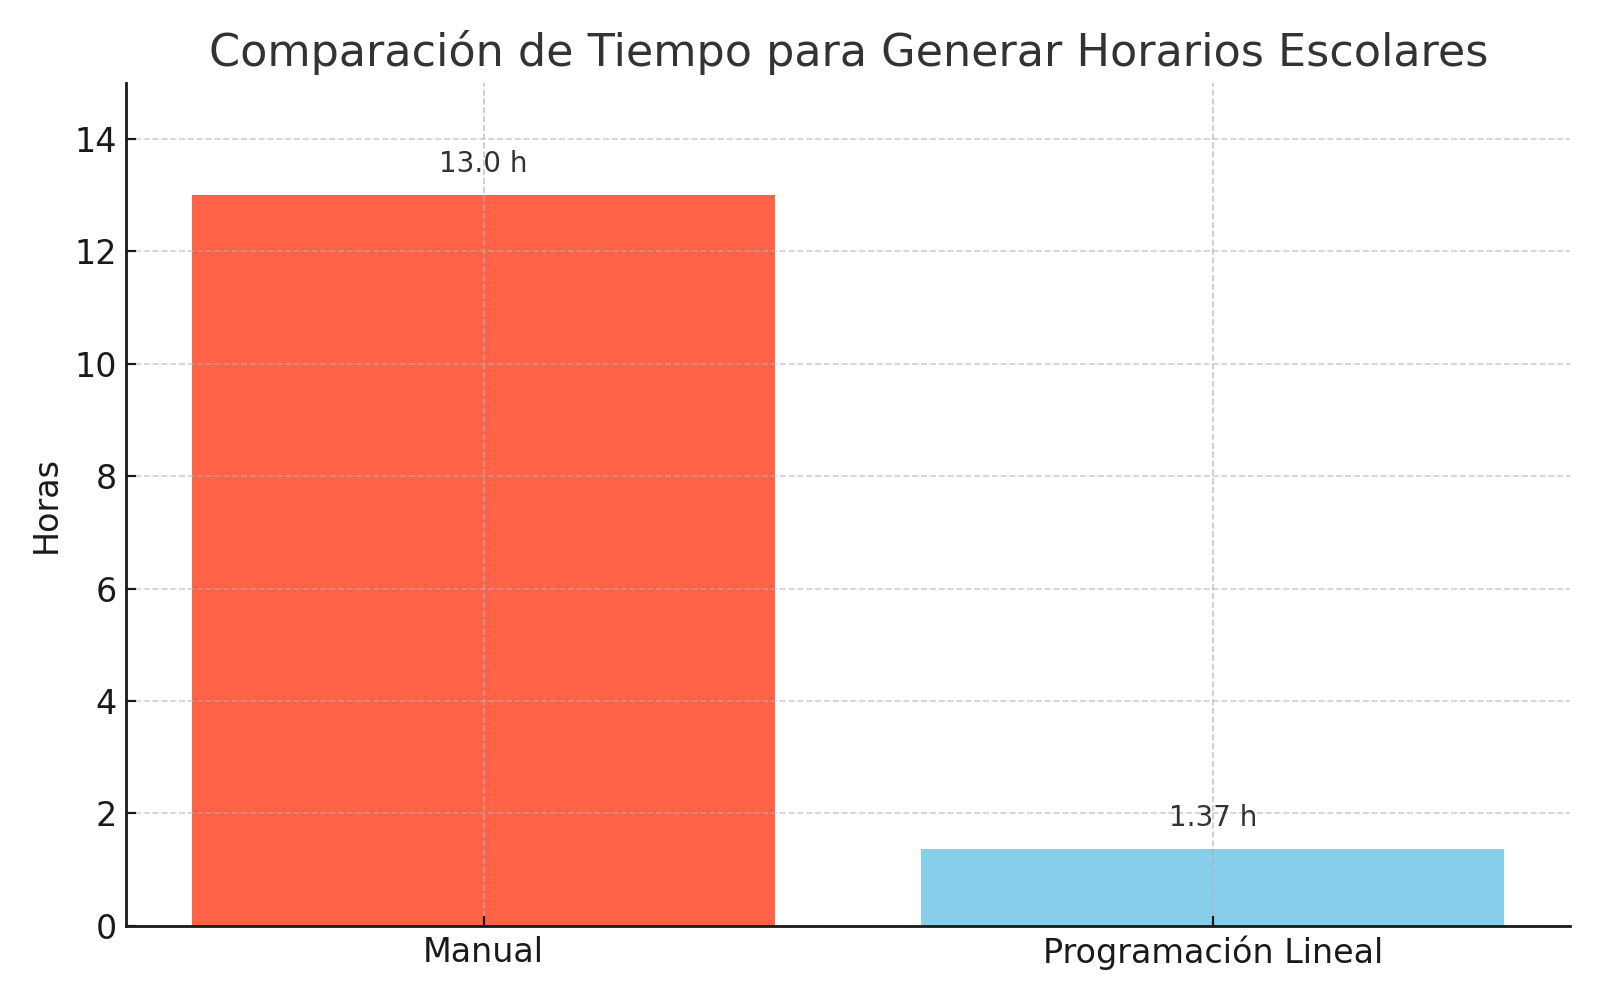
\includegraphics[width=0.7\linewidth]{comparacion_tiempos_horarios.png}
    \caption{Comparación de tiempo: método manual vs. programación lineal}
\end{figure}

  \end{itemize}
\end{frame}

% 6. Conclusión
\begin{frame}{Conclusiones}
  \begin{itemize}
    \item Se redujo significativamente el tiempo de generación de horarios.
    \item Mayor precisión y menos errores.
    \item La programación lineal es muy útil en la planificación escolar.
    \item Se demostró que herramientas como Excel también pueden optimizar.
  \end{itemize}
\end{frame}

\end{document}

